\documentclass[ignorenonframetext,]{beamer}
\setbeamertemplate{caption}[numbered]
\setbeamertemplate{caption label separator}{: }
\setbeamercolor{caption name}{fg=normal text.fg}
\beamertemplatenavigationsymbolsempty
\usepackage{lmodern}
\usepackage{amssymb,amsmath}
\usepackage{ifxetex,ifluatex}
\usepackage{fixltx2e} % provides \textsubscript
\ifnum 0\ifxetex 1\fi\ifluatex 1\fi=0 % if pdftex
  \usepackage[T1]{fontenc}
  \usepackage[utf8]{inputenc}
\else % if luatex or xelatex
  \ifxetex
    \usepackage{mathspec}
  \else
    \usepackage{fontspec}
  \fi
  \defaultfontfeatures{Ligatures=TeX,Scale=MatchLowercase}
\fi
\usefonttheme{structurebold}
% use upquote if available, for straight quotes in verbatim environments
\IfFileExists{upquote.sty}{\usepackage{upquote}}{}
% use microtype if available
\IfFileExists{microtype.sty}{%
\usepackage{microtype}
\UseMicrotypeSet[protrusion]{basicmath} % disable protrusion for tt fonts
}{}
\newif\ifbibliography
\usepackage{color}
\usepackage{fancyvrb}
\newcommand{\VerbBar}{|}
\newcommand{\VERB}{\Verb[commandchars=\\\{\}]}
\DefineVerbatimEnvironment{Highlighting}{Verbatim}{commandchars=\\\{\}}
% Add ',fontsize=\small' for more characters per line
\usepackage{framed}
\definecolor{shadecolor}{RGB}{248,248,248}
\newenvironment{Shaded}{\begin{snugshade}}{\end{snugshade}}
\newcommand{\KeywordTok}[1]{\textcolor[rgb]{0.13,0.29,0.53}{\textbf{{#1}}}}
\newcommand{\DataTypeTok}[1]{\textcolor[rgb]{0.13,0.29,0.53}{{#1}}}
\newcommand{\DecValTok}[1]{\textcolor[rgb]{0.00,0.00,0.81}{{#1}}}
\newcommand{\BaseNTok}[1]{\textcolor[rgb]{0.00,0.00,0.81}{{#1}}}
\newcommand{\FloatTok}[1]{\textcolor[rgb]{0.00,0.00,0.81}{{#1}}}
\newcommand{\ConstantTok}[1]{\textcolor[rgb]{0.00,0.00,0.00}{{#1}}}
\newcommand{\CharTok}[1]{\textcolor[rgb]{0.31,0.60,0.02}{{#1}}}
\newcommand{\SpecialCharTok}[1]{\textcolor[rgb]{0.00,0.00,0.00}{{#1}}}
\newcommand{\StringTok}[1]{\textcolor[rgb]{0.31,0.60,0.02}{{#1}}}
\newcommand{\VerbatimStringTok}[1]{\textcolor[rgb]{0.31,0.60,0.02}{{#1}}}
\newcommand{\SpecialStringTok}[1]{\textcolor[rgb]{0.31,0.60,0.02}{{#1}}}
\newcommand{\ImportTok}[1]{{#1}}
\newcommand{\CommentTok}[1]{\textcolor[rgb]{0.56,0.35,0.01}{\textit{{#1}}}}
\newcommand{\DocumentationTok}[1]{\textcolor[rgb]{0.56,0.35,0.01}{\textbf{\textit{{#1}}}}}
\newcommand{\AnnotationTok}[1]{\textcolor[rgb]{0.56,0.35,0.01}{\textbf{\textit{{#1}}}}}
\newcommand{\CommentVarTok}[1]{\textcolor[rgb]{0.56,0.35,0.01}{\textbf{\textit{{#1}}}}}
\newcommand{\OtherTok}[1]{\textcolor[rgb]{0.56,0.35,0.01}{{#1}}}
\newcommand{\FunctionTok}[1]{\textcolor[rgb]{0.00,0.00,0.00}{{#1}}}
\newcommand{\VariableTok}[1]{\textcolor[rgb]{0.00,0.00,0.00}{{#1}}}
\newcommand{\ControlFlowTok}[1]{\textcolor[rgb]{0.13,0.29,0.53}{\textbf{{#1}}}}
\newcommand{\OperatorTok}[1]{\textcolor[rgb]{0.81,0.36,0.00}{\textbf{{#1}}}}
\newcommand{\BuiltInTok}[1]{{#1}}
\newcommand{\ExtensionTok}[1]{{#1}}
\newcommand{\PreprocessorTok}[1]{\textcolor[rgb]{0.56,0.35,0.01}{\textit{{#1}}}}
\newcommand{\AttributeTok}[1]{\textcolor[rgb]{0.77,0.63,0.00}{{#1}}}
\newcommand{\RegionMarkerTok}[1]{{#1}}
\newcommand{\InformationTok}[1]{\textcolor[rgb]{0.56,0.35,0.01}{\textbf{\textit{{#1}}}}}
\newcommand{\WarningTok}[1]{\textcolor[rgb]{0.56,0.35,0.01}{\textbf{\textit{{#1}}}}}
\newcommand{\AlertTok}[1]{\textcolor[rgb]{0.94,0.16,0.16}{{#1}}}
\newcommand{\ErrorTok}[1]{\textcolor[rgb]{0.64,0.00,0.00}{\textbf{{#1}}}}
\newcommand{\NormalTok}[1]{{#1}}
\usepackage{graphicx,grffile}
\makeatletter
\def\maxwidth{\ifdim\Gin@nat@width>\linewidth\linewidth\else\Gin@nat@width\fi}
\def\maxheight{\ifdim\Gin@nat@height>\textheight0.8\textheight\else\Gin@nat@height\fi}
\makeatother
% Scale images if necessary, so that they will not overflow the page
% margins by default, and it is still possible to overwrite the defaults
% using explicit options in \includegraphics[width, height, ...]{}
\setkeys{Gin}{width=\maxwidth,height=\maxheight,keepaspectratio}

% Prevent slide breaks in the middle of a paragraph:
\widowpenalties 1 10000
\raggedbottom

\AtBeginPart{
  \let\insertpartnumber\relax
  \let\partname\relax
  \frame{\partpage}
}
\AtBeginSection{
  \ifbibliography
  \else
    \let\insertsectionnumber\relax
    \let\sectionname\relax
    \frame{\sectionpage}
  \fi
}
\AtBeginSubsection{
  \let\insertsubsectionnumber\relax
  \let\subsectionname\relax
  \frame{\subsectionpage}
}

\setlength{\emergencystretch}{3em}  % prevent overfull lines
\providecommand{\tightlist}{%
  \setlength{\itemsep}{0pt}\setlength{\parskip}{0pt}}
\setcounter{secnumdepth}{0}
\definecolor{links}{HTML}{800080}
\hypersetup{colorlinks,linkcolor=,urlcolor=links}

\title{Web Data Collection with R}
\subtitle{HTML Forms}
\author{Peter Meißner / 2016-02-29 -- 2016-03-04 / ECPR WSMT}
\date{}

\begin{document}
\frame{\titlepage}

\begin{frame}
\tableofcontents[hideallsubsections]
\end{frame}

\section{HTML Forms}\label{html-forms}

\begin{frame}[fragile]{How HTML forms work}

\begin{itemize}
\tightlist
\item
  HTML forms are a collection of HTML nodes/tags
  (\texttt{\textless{}form\textgreater{},\ \textless{}input\textgreater{},\ \textless{}select\textgreater{},\ \textless{}textfield\textgreater{}})
\item
  those elements

  \begin{itemize}
  \tightlist
  \item
    collect data as textfields, radio buttons, calenders, checkmarks,
    \ldots{}.
  \item
    describe location
  \item
    and HTTP method with which
  \item
    data is to be send
  \end{itemize}
\item
  html forms are a way to interact with the server
\item
  \url{http://www.r-datacollection.com/materials/html/InputTypes.html}
\end{itemize}

\end{frame}

\begin{frame}{HTML forms}

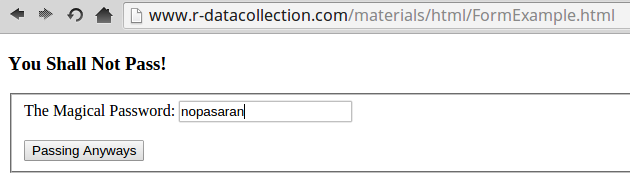
\includegraphics{fig/nopasaran.png}

\end{frame}

\begin{frame}[fragile]{HTML forms}

\begin{Shaded}
\begin{Highlighting}[]
\DataTypeTok{<!DOCTYPE }\NormalTok{html}\DataTypeTok{>}
\KeywordTok{<html>}
  \KeywordTok{<head>}
  \KeywordTok{<title>}\NormalTok{No pasaran!}\KeywordTok{</title>}
  \KeywordTok{</head>}
  \KeywordTok{<body>}
    \KeywordTok{<h3}\OtherTok{ id=}\StringTok{"heading"} \KeywordTok{>}\NormalTok{You Shall Not Pass!}\KeywordTok{</h3>}
    \KeywordTok{<form}\OtherTok{ name=}\StringTok{"submitPW"}\OtherTok{ action=}\StringTok{"Passed.html"}\OtherTok{ method=}\StringTok{"get"}\KeywordTok{>}
      \KeywordTok{<fieldset>}
        \NormalTok{The Magical Password: }
        \KeywordTok{<input}\OtherTok{ name=}\StringTok{"pw"}\OtherTok{ type=}\StringTok{"text"}\OtherTok{ value=}\StringTok{""}\KeywordTok{>}
        \KeywordTok{<input}\OtherTok{ type=}\StringTok{"submit"}\OtherTok{ value=}\StringTok{"Passing Anyways"}\KeywordTok{>}
      \KeywordTok{</fieldset>}
    \KeywordTok{</form>}
  \KeywordTok{</body>}
\KeywordTok{</html>}
\end{Highlighting}
\end{Shaded}

\end{frame}

\begin{frame}[fragile]{HTML forms}

important information about HTML form to fill out and send forms

\begin{itemize}
\tightlist
\item
  which method does it demand - POST or GET -\textgreater{} use httr's
  \texttt{GET()} and \texttt{POST()} respectively
\item
  if method POST is used, is a enctype given
  (`application/x-www-form-urlencoded' is the default and
  `multipart/form-data' the one that should be used when uploading any
  kind of file) -\textgreater{} use httr function's
  \texttt{encode="form"} or \texttt{encode="multipart"}
\item
  which are the inputs (inputs can be ,

  , there parameter name is given by the name attribute) -\textgreater{}
  use either httr's
  \texttt{GET(...,\ query=list(param1="value",\ param2="value2"))} or
  \texttt{POST(...,\ )}
\item
  where should the data be end to (the value of the action attribute)
  -\textgreater{} use it as URL in your function call
\end{itemize}

\end{frame}

\end{document}
